% Figure: Pipeline Current vs Recommended State
% Comparison of deployment pipeline practices

\begin{figure}[htbp]
    \centering
    \resizebox{0.9\textwidth}{!}{%
    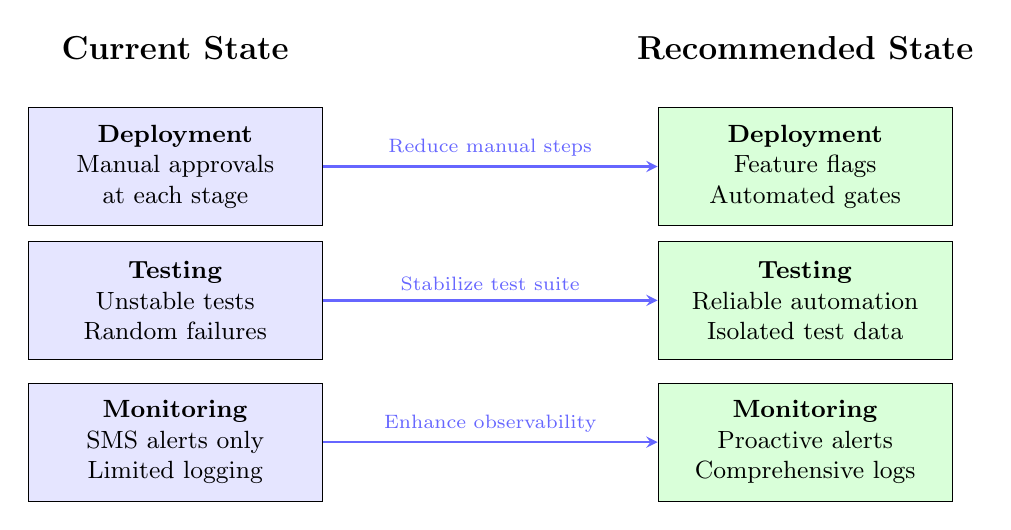
\begin{tikzpicture}[
        box/.style={rectangle, draw, fill=blue!10, text width=3.5cm, align=center, minimum height=1.5cm, font=\small},
        goodbox/.style={rectangle, draw, fill=green!15, text width=3.5cm, align=center, minimum height=1.5cm, font=\small},
        title/.style={font=\bfseries\large},
        arrow/.style={->, >=stealth, thick}
    ]

    % Current State (Left)
    \node[title] (current) at (0,5) {Current State};

    \node[box] (c1) at (0,3.5) {\textbf{Deployment}\\Manual approvals\\at each stage};
    \node[box] (c2) at (0,1.8) {\textbf{Testing}\\Unstable tests\\Random failures};
    \node[box] (c3) at (0,0) {\textbf{Monitoring}\\SMS alerts only\\Limited logging};

    % Recommended State (Right)
    \node[title] (recommended) at (8,5) {Recommended State};

    \node[goodbox] (r1) at (8,3.5) {\textbf{Deployment}\\Feature flags\\Automated gates};
    \node[goodbox] (r2) at (8,1.8) {\textbf{Testing}\\Reliable automation\\Isolated test data};
    \node[goodbox] (r3) at (8,0) {\textbf{Monitoring}\\Proactive alerts\\Comprehensive logs};

    % Connecting arrows with improvement labels
    \draw[arrow, blue!60] (c1) -- node[above, font=\scriptsize] {Reduce manual steps} (r1);
    \draw[arrow, blue!60] (c2) -- node[above, font=\scriptsize] {Stabilize test suite} (r2);
    \draw[arrow, blue!60] (c3) -- node[above, font=\scriptsize] {Enhance observability} (r3);

    \end{tikzpicture}%
    }
    \caption{Comparison of current and recommended pipeline practices. Current state relies on manual approvals and reactive monitoring. Recommended improvements focus on automation, test stability, and comprehensive observability to enable faster feedback and reduce operational overhead.}
    \label{fig:jawad-pipeline-comparison}
\end{figure}
